\documentclass[12pt,titlepage]{article}
\usepackage[section]{placeins}
\usepackage{graphicx}
\usepackage{svg}
%\usepackage{graphics}
\usepackage{epsfig}
\usepackage{amsmath}
\usepackage{amssymb}
\usepackage{amsthm}
\usepackage{booktabs}
\usepackage{stmaryrd}
\usepackage{url}
\usepackage{float}
%\usepackage{longtable}
\usepackage[figuresright]{rotating}

\usepackage{polski}
\usepackage[utf8]{inputenc}
\usepackage[T1]{fontenc}

\usepackage{geometry}
\usepackage{pslatex}
%\usepackage{ulem}

\usepackage{listings}
\usepackage{url}
%\usepackage{Here}

\usepackage{color}
\numberwithin{equation}{section}

\definecolor{szary}{gray}{0.1}% jasnoszary

% \setlength{\textwidth}{400pt}

\lstset{numbers=left,
			numberstyle=\tiny, 
			basicstyle=\scriptsize\ttfamily, 
			breaklines=true, 
			captionpos=b, 
			tabsize=2}

\usepackage[ruled,vlined,linesnumbered]{algorithm2e}

\vfuzz2pt % Don't report over-full v-boxes if over-edge is small
\hfuzz2pt % Don't report over-full h-boxes if over-edge is small


\newcommand{\RR}{\mathbb{R}}
\newcommand{\NN}{\mathbb{N}}
\newcommand{\QQ}{\mathbb{Q}}
\newcommand{\ZZ}{\mathbb{Z}}
\newcommand{\TAB}{\hspace{0.50cm}}
\newcommand{\IFF}{\leftrightarrow}
\newcommand{\IMP}{\rightarrow}

\newcommand{\PRZYKLAD}[1]{\par \noindent{\color{blue}PRZYKŁAD:}\\ {\color{szary}#1}\par}

\newtheorem{theorem}{Twierdzenie}[section]
\newtheorem{lemma}{Lemat}[section]
\newtheorem{example}{Przykład}[section]
\newtheorem{corollary}{Wniosek}[section]
\newtheorem{definition}{Definicja}[section]




\begin{document}
\pagestyle{empty} %To jest strona tytułowa, bez numeracji

\begin{titlepage}
\vspace*{\fill}
\begin{center}
\begin{picture}(300,510)
  \put( 10,520){\makebox(0,0)[l]{\normalsize \bf \textsc{Wydział Podstawowych Problemów Techniki}}}
  \put( 10,500){\makebox(0,0)[l]{\normalsize \bf \textsc{Politechniki Wrocławskiej}}}
  \put( 50,300){\makebox(0,0)[l]{\Large  \bf \textsc{Efektywne wyliczanie}}}
  \put( 50,280){\makebox(0,0)[l]{\Large  \bf \textsc{wartości zagrożonej ryzykiem}}}
  \put( 50,260){\makebox(0,0)[l]{\Large  \bf \textsc{z użyciem systemu Akka}}}
  \put(100,230){\makebox(0,0)[l]{\normalsize     \textsc{Michał Kordel}}}

  \put(170, 80){\makebox(0,0)[l]{\large  {Praca inżynierska napisana}}}
  \put(170, 60){\makebox(0,0)[l]{\large  {pod kierunkiem}}}
  \put(170, 40){\makebox(0,0)[l]{\large \bf  {dr inż. Jakuba Lemiesza}}}

  \put(100,-80){\makebox(0,0)[bl]{\large \bf \textsc{Wrocław 2017}}}
\end{picture}
\end{center}
\vspace*{\fill}
\end{titlepage}

\tableofcontents

\newpage

\pagestyle{headings}  %Zaczynamy właściwą część dokumentu

\section{Wstęp ogólny} 
Celem realizowanej pracy inżynierskiej będzie zaprojektowanie i zaimplementowanie klastra obliczeniowego, który będzie wyliczał Wartość Zagrożoną ryzykiem (ang. Value at Risk, $VaR$) metodą symulacji Monte Carlo. System Akka jest efektywnym narzędziem do implementacji obliczeń rozproszonych na platformie JVM. Oparty on jest na modelu aktorów, ten model współbieżności jest asynchroniczny i polega na przesyłaniu wiadomości pomiędzy podstawowymi jednostkami obliczeniowymi - aktorami. W tym modelu żadne dane nie są współdzielone, a zmienne synchronizacyjne takie jak mutexy czy semafory nie są potrzebne. W systemie Akka aktorzy mogą być wykonywani zarówno w obrębie jednej, jak i wielu maszyn bez ingerencji w kod źródłowy samych aktorów. Dodatkową cechą tego systemu jest hierarchiczność samych aktorów - każdy aktor posiada jednego aktora-rodzica który nadzoruje jego pracę. Model aktorów jak i system Akka zostaną bardziej szczegółowo omówione w rozdziale 4. 

Value at Risk jest miarą ryzyka inwestycyjnego wyliczaną dla zadanego przedziału czasowego $t$. Może być wyznaczana dla pojedynczych instrumentów finansowych (np. akcje, obligacje, kontrakty terminowe) jak i dla całych portfeli składających się z tychże instrumentów. Niech $X$ - zmienna losowa oznaczająca wartość portfela po upływie czasu $t$ oraz niech $\alpha$ - założony poziom ufności. Mamy
$$VaR_{\alpha}=inf\{ x\in \mathbb{R}:P(X+x<0) <  1-\alpha \}.$$
Intuicyjnie jest to maksymalna strata wartości portfela jaka może zostać poniesiona w czasie $t$ przy założonym poziomie ufności $\alpha$. Zauważmy, że powyższa nie jest konstruktywna - mówi jedynie jaki warunek $VaR$ musi spełniać, nie podając sposobu jej wyliczania. Opisy podstawowych algorytmów wyznaczania $VaR$ znajdują się w rozdziale 3.


\newpage
\section{Wykorzystywane oznaczenia i narzędzia matematyczne}
Należy zdefiniować podstawowe formalizmy wykorzystywane przy algorytmach wyznaczania $VaR$. 






\subsection{Problem wyznaczania macierzy transformacji} \label{mtransformacji}
Dane są $n$-elementowy wektor nieskorelowanych zmiennych losowych $X$ pochodzących ze standardowego rozkładu normalnego oraz macierz kowariancji $\Sigma$

\begin{equation} 
X=
\begin{bmatrix}
 x_1 \\ 
 x_2 \\
\vdots \\
x_n
\end{bmatrix}
,\Sigma=\begin{bmatrix}
\sigma_{11} & \sigma_{12} & \hdots & \sigma_{1n} \\ 
\sigma_{21} & \sigma_{22} & \hdots & \sigma_{2n} \\
\vdots & \vdots & \ddots & \vdots\\
\sigma_{n1} & \sigma_{n2} & \hdots & \sigma_{nn}
\end{bmatrix}.
\end{equation} 
Wartość oczekiwana jest  równa 0 dla każdego elementu wektora X, innymi słowy

\begin{equation}
\left \langle X \right \rangle = \vec{0},
\end{equation} 
a wariancja każdego elementu wektora będzie równa 1, co można zapisać jako


\begin{equation}
\left \langle X \cdot X^T \right \rangle = I
\end{equation} 
gdzie przez $I$ rozumie się macierz jednostkową. Symbolem $Y$ oznaczono $n$-elementowy wektor zmiennych losowych, których korelacja wyrażona została przy pomocy macierzy kowariancji $\Sigma$


\begin{equation}\label{eq:yysigma}
\left \langle Y \cdot Y^T \right \rangle = \Sigma.
\end{equation} 
Zadaniem jest znalezienie macierzy transformacji $C$ takiej, że spełniona jest równość

\begin{equation}\label{eq:ycx}
Y=C \cdot X.
\end{equation} 
W równaniu \eqref{eq:yysigma} można zastosować podstawienie \eqref{eq:ycx}. Wówczas

\begin{equation}\label{eq:cct}
\Sigma = \left \langle Y \cdot Y^T \right \rangle = \left \langle C \cdot X \cdot (C \cdot X)^T \right \rangle =
\left \langle C \cdot X \cdot X^T \cdot C^T \right \rangle =  C \cdot \left \langle X \cdot X^T \right \rangle \cdot C^T =
C \cdot I \cdot C^T = C \cdot C^T.
\end{equation} 
Należy zatem wyznaczyć macierz $C$ spełniającą równość $C \cdot C^T = \Sigma$. Takie równanie można rozwiązać m.in. algorytmem dekompozycji Choleskiego. Istnieje jednak inne efektywne podejście. Opiera się ono na diagonalizacji macierzy kowariancji. Wówczas równanie przedstawia się następująco 

\begin{equation}\label{eq:pdeltap}
\Sigma=P\Delta P^T=P \Delta^{\frac{1}{2}} \Delta^{\frac{1}{2}} P^T \stackrel{*}{=}
P   \Delta^{\frac{1}{2}}  (\Delta^{\frac{1}{2}})^T   P^T =
P   \Delta^{\frac{1}{2}}  ( P   \Delta^{\frac{1}{2}} )^T.
\end{equation} 
W przejściu oznaczonym znakiem $(*)$ został wykorzystany fakt, że transponowana macierz diagonalna pozostaje tą samą macierzą. Porównując równania \eqref{eq:cct} oraz \eqref{eq:pdeltap} można dokonać podstawienia


\begin{equation}\label{eq:cpdeltafrac}
C  =P  \Delta^{\frac{1}{2}}.
\end{equation} 























\section{Omówienie podstawowych metod}
Istnieją trzy podstawowe metody obliczania $VaR$: metoda wariancji-kowariancji, metoda symulacji historycznej oraz metoda symulacji Monte Carlo. Ta ostatnia wymaga największego nakładu mocy obliczeniowej.



\subsection{Metoda wariancji-kowariancji}


Metoda wariancji-kowariancji jest najprostsza i posiada najmniejszą złożoność obliczeniową. Na początku przyjmowane jest założenie o normalności rozkładu zmian cen. Dodatkowo zakładane jest że średnia $\mu$ rozkładu zmian cen jest równa 0. Jest to tylko przybliżenie rzeczywistych rozkładów zmian cen, jednak w przypadku portfeli prostych, tj. niezawierających instrumentów pochodnych, jest to wystarczająco dobre przybliżenie. 

Rozważania należy rozpocząć od portfela składającego się tylko z jednej pozycji, czyli zawierającego tylko jeden typ instrumentów finansowych. Ustalmy przedział czasowy pomiędzy badanymi zmianami cen $t=24h$. Niech $V$ oznacza wartość portfela inwestycyjnego, $\mu$ oznacza średnią rozkładu zmian cen, zaś $\sigma^{2}$ jest wariancją tego rozkładu. Funkcję odwrotnej dystrybuanty dla rozkładu normalnego definiujemy wzorem 




\begin{equation} 
\Phi_{\mu,\sigma^{2}}^{-1}(\alpha)=\mu+\sigma \sqrt{2} erf^{-1}(2\alpha-1)
\end{equation} 
gdzie $erf^{-1}$ jest odwrotnością funkcji błędu. Korzystając z początkowego założenia o zerowej średniej rozkładu mamy
$$\Phi_{\mu=0,\sigma^{2}}^{-1}(\alpha)=\sigma \sqrt{2} erf^{-1}(2\alpha-1)$$



Symbolem $VaR^{rel}$ oznaczamy względną wartość narażoną na ryzyko.Względna wartość narażona na ryzyko nie uwzględnia wartości pozycji w portfelu, więc graniczna strata jest tu wyrażona nie jako konkretna kwota, lecz jako liczba z przedziału $(0,1)$ oznaczająca część portfela narażoną na ryzyko. $VaR^{rel}$ dla pojedynczej pozycji przy poziomie tolerancji $\alpha$ jest zdefiniowane jako

$$VaR_{\alpha}^{rel}   =\Phi_{\mu=0,\sigma^{2}}^{-1}(\alpha).$$

Wizualizacja tej wartości jest dość intuicyjna. Mając dany wykres gęstości prawdopodobieństwa, $VaR^{rel}$ będzie takim punktem na osi $OX$, że pole pod wykresem na przedziale $(-\infty,VaR^{rel})$  będzie równe $\alpha$. Dla przykładu, weźmy rozkład zmian cen złota dla przedziału czasowego $t=24h$. Mamy $\mu=0$ oraz $\sigma=0.005532$. Dodatkowo przyjmijmy $\alpha=0.05$. Wykres gęstości prawdopodobieństwa dla tego rozkładu będzie następujący

\begin{figure}[H]
\begin{center}
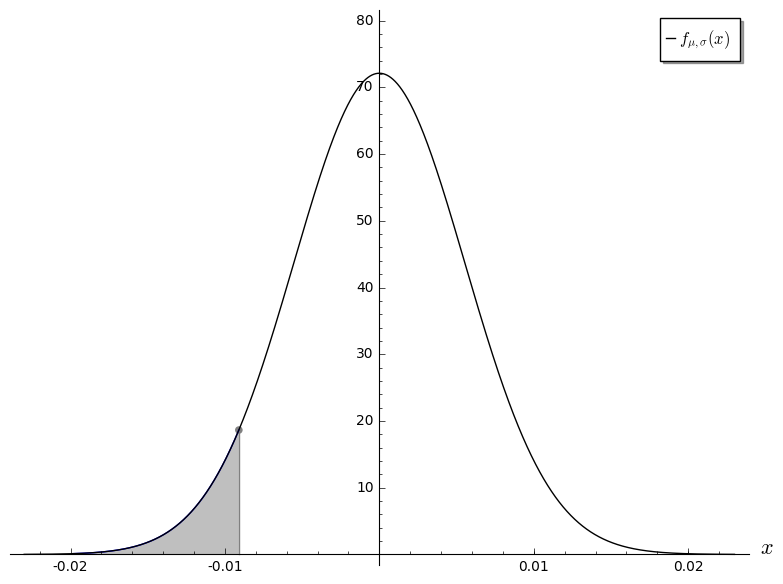
\includegraphics[scale=0.5]{chart1.png}
\end{center}
\caption{Rozkład względnych zmian cen złota z zacienionym poziomem tolerancji} \label{czynnosci_GD}
\end{figure} 


Oznaczmy teraz $k$ - kwantyl rzędu $\alpha$ dla standardowego rozkładu normalnego, czyli bardziej formalnie 
$$k=\Phi_{\mu=0,\sigma^{2}=1}^{-1}(\alpha)=\sqrt{2} erf^{-1}(2\alpha-1).$$
Możemy więc zastosować przekształcenie
$$VaR_{\alpha}^{rel}   =\sigma \sqrt{2} erf^{-1}(2\alpha-1)=\sigma \cdot k$$
z którego wynika że $VaR_{\alpha}^{rel}$ wyliczyć można korzystając z tablic kwantyli standardowego rozkładu normalnego. Dla $\alpha=0.05$ mamy $k=-1.645$. Odchylenie standardowe $\sigma=0.005532$. Zatem
$$VaR_{\alpha}^{rel}=\sigma \cdot k= 0.005532 \cdot (-1.645)=-0.0091.$$

\noindent Bezwzględną wartość narażoną na ryzyko obliczamy korzystając ze wzoru
$$VaR = V \cdot |VaR^{rel}|.$$
Jeśli ustalimy $V=10000\$$ to otrzymamy $VaR = 10000\$ \cdot |-0.0091| = 91\$ $.

Rozważmy teraz przypadek gdy w portfelu inwestycyjnym znajduje się więcej niż jedna pozycja. Weźmy portfel $n$-instrumentowy. Niech
$$V=\begin{bmatrix}
 v_1 \\ 
 v_2 \\
\vdots \\
v_n
\end{bmatrix}$$
będzie wektorem wartości kolejnych instrumentów w portfelu.

Założyliśmy wcześniej, że rozkład zmian cen każdego instrumentu w portfelu jest rozkładem normalnym. Ponadto zmiany te są wzajemnie ze sobą skorelowane. Zmiana wartości całego portfela jest kombinacją liniową zmian wartości poszczególny instrumentów, mamy więc do czynienia z wielowymiarowym rozkładem normalnym. Wielowymiarowy rozkład normalny zadany jest wektorem wartości średnich rozkładów $\mu$ oraz kwadratową macierzą kowariancji $\Sigma$
$$\mu=\begin{bmatrix}
 \mu_1 \\ 
 \mu_2 \\
\vdots \\
\mu_n
\end{bmatrix},\Sigma=\begin{bmatrix}
\sigma_{11} & \sigma_{12} & \hdots & \sigma_{1n} \\ 
\sigma_{21} & \sigma_{22} & \hdots & \sigma_{2n} \\
\vdots & \vdots & \ddots & \vdots\\
\sigma_{n1} & \sigma_{n2} & \hdots & \sigma_{nn}
\end{bmatrix}. $$

Ze względu na początkowe założenia wektor $\mu$ będzie tutaj wektorem zerowym. Korzystając z własności wielowymiarowego rozkładu normalnego możemy obliczyć wariancję rozkładu zmian wartości całego portfela 


$$ \sigma_{Portfela}^2 = V^T  \cdot \Sigma \cdot V =  \begin{bmatrix}
 v_1 & v_2 & \hdots & v_n
\end{bmatrix} 
\cdot
\begin{bmatrix}
\sigma_{11} & \sigma_{12} & \hdots & \sigma_{1n} \\ 
\sigma_{21} & \sigma_{22} & \hdots & \sigma_{2n} \\
\vdots & \vdots & \ddots & \vdots\\
\sigma_{n1} & \sigma_{n2} & \hdots & \sigma_{nn}
\end{bmatrix}  
\cdot
\begin{bmatrix}
 v_1 \\ 
 v_2 \\
\vdots \\
v_n
\end{bmatrix}
=\sum_{i=1}^{n}\sum_{j=1}^{n}w_i w_j \sigma_{ij}.
$$


Mając wyznaczoną wariancję zmian wartości całego portfela, traktujemy ten rozkład jako jednowymiarowy. Można zatem wyznaczyć $VaR^{rel}$
$$VaR^{rel}=\sigma_{Portfela} \cdot k,$$
a także bezwzględną $VaR$
$$VaR = (\sum_{i=1}^{n}v_i) \cdot VaR^{rel}.$$.



\subsection{Metoda symulacji historycznej}



Metoda symulacji historycznej nie zakłada normalności rozkładu zmian cen, w ogóle nie są podejmowane jakiekolwiek wstępne założenia co do tego rozkładu. Rozkład ten opiera się wyłącznie na danych historycznych. Algorytm jako dane wejściowe przyjmuje względne zmiany cen aktywów, tworzy szereg wartości portfela. Mając szereg wartości portfela tworzymy szereg różnic pomiędzy wartością portfela każdego dnia a początkową wartością portfela. Szereg ten sortujemy rosnąco. Z tego szeregu wyznaczając odpowiedni (na podstawie założonego poziomu ufności) kwantyl otrzymujemy $VaR$.\\



\subsection{Metoda symulacji Monte Carlo}


Od metody symulacji historycznej  metoda symulacji Monte Carlo różni się tym, że nie posiadamy szeregów zmian cen. Generujemy je za pomocą generatora liczb pseudolosowych. Zakładamy normalność rozkładów zmian cen dla każdego z instrumentów portfelu. Implikuje to fakt, że rozkład wartości zmian cen dla całego portfela również będzie normalny, ponieważ zmiana wartości portfela jest kombinacją liniową wartości poszczególnych instrumentów. 

%eeee wektor Y
Załóżmy że w portfelu inwestycyjnym znajduje się $n$ różnych pozycji.Niech $X=\begin{bmatrix}
 X_1 & X_2 & \hdots & X_n
\end{bmatrix}^T $ będzie wektorem nieskorelowanych zmiennych losowych ze standardowego rozkładu normalnego. Ponadto, niech $\Sigma$ będzie macierzą kowariancji rozkładu zmian cen, ustaloną na podstawie historycznych zmian cen, a $Y$ niech będzie takim wektorem zmiennym losowych o rozkładzie normalnym takim, że jego macierzą kowariancji jest $\Sigma$. Aby wykonać symulację Monte Carlo, należy znaleźć macierz transformacji $C$, czyli macierz spełniającą równanie 

\begin{equation}
    Y=C \cdot X.
\end{equation}
Metoda wyznaczania takiej macierzy przedstawiona jest w rozdziale \ref{mtransformacji}. Metoda zwraca wynik w postaci iloczynu dwóch macierzy

\begin{equation}
    C=P \cdot \Delta^{\frac{1}{2}}.
\end{equation}
Macierze $P$ i $\Delta$ powstały jako efekt diagonalizacji macierzy $\Sigma$, tj. $\Sigma=P \cdot \Delta \cdot P^{-1}$, gdzie  $P$ jest macierzą przejścia, a $\Delta$ macierzą diagonalną. Jako że $P$ jest macierzą przejścia to możemy ją przedstawić jako macierz kolumnową, której kolumny $P_1, \hdots, P_n$ są wektorami własnymi macierzy $\Sigma$
\begin{equation}
    P=\begin{bmatrix} P_1 & \vdots & P_2 & \vdots  & \hdots & \vdots & P_n \end{bmatrix}.
\end{equation}
Wektor $P_i$ nazywamy wektorem własnym macierzy kowariancji dla instrumentu $i$, symbolem $P_{i}[j]$ oznaczamy $j$-ty element wektora własnego $P_i$. Ponadto zauważmy, że macierz $\Delta^{\frac{1}{2}}$ można wyliczyć z macierzy $\Delta$ korzystając własności potęgowania macierzy diagonalnych



\begin{equation}
\Delta^{\frac{1}{2}}=\begin{bmatrix} \sqrt{\Delta_1} &  \cdots &0 \\
\vdots & \ddots  & \vdots \\ 0& \cdots & \sqrt{\Delta_n} \end{bmatrix}.
\end{equation} 
Algorytm zaczyna pracę od wygenerowania dla każdego instrumentu w portfelu szereg liczb pseudolosowych (standardowo 10000 liczb) z rozkładu normalnego o parametrach $\mu=0,\sigma^2=1$. Wprowadźmy następujące oznaczenie $X_j(k)$ - realizacja zmiennej losowej $X_j$ dla $k$-tego losowania. Innymi słowy dla instrumentu z indeksem $j$ w szeregu liczb pseudolosowych $k$-ty element będzie równy $X_j(k)$. Dla dowolnego $k \in \left \{1, \hdots, 10000 \right \} $ mamy



\begin{equation} \label{eq:ynk}
Y(k)=
    \begin{bmatrix}
 Y_1(k) \\ 
\vdots \\
Y_n(k)
\end{bmatrix} =
C \cdot \begin{bmatrix}
 X_1(k) \\ 
\vdots \\
X_n(k)
\end{bmatrix} =
    \begin{bmatrix}
    \begin{bmatrix}P_1[1] \\ \vdots \\ P_1[n]\end{bmatrix} &
    \hdots &
    \begin{bmatrix}P_n[1] \\ \vdots \\ P_n[n]\end{bmatrix} 
\end{bmatrix}
    \cdot
\begin{bmatrix} \sqrt{\Delta_1} &  \cdots &0 \\
\vdots & \ddots  & \vdots \\ 0& \cdots & \sqrt{\Delta_n} \end{bmatrix}
    \cdot 
\begin{bmatrix}
 X_1(k) \\ 
\vdots \\
X_n(k)
\end{bmatrix}
\end{equation}
Wektor $Y(k)$ nazywamy wektorem skorelowanych względnych zmian cen. Stosując wzory na mnożenie macierzy przy ustalonym wcześniej $k$, dla każdego $j \in \left \{1, \hdots, n \right \} $ mamy
 
 
 \begin{equation}
     Y_j(k)=\sum_{i=1}^{n}P_i[j] \cdot \sqrt{\Delta_j}\cdot X_j(k).
 \end{equation}
Zauważmy, że każdy wektor $Y(k)$ można wyznaczyć niezależnie od pozostałych, co jest istotne z punktu widzenia przetwarzania w klastrze, ponieważ każdy węzeł klastra będzie mógł wyliczać wektory niezależnie, nie oczekując na pozostałe węzły. Choć ten fakt nie zostanie w praktyce wykorzystany - bo wówczas stopień rozproszenia obliczeń przyniósłby więcej strat niż korzyści - nawet pojedyncze elementy wektorów $Y(k)$ można wyznaczać niezależnie.
Zwróćmy jeszcze uwagę na złożoność obliczeniową takiej symulacji bez zagłębiania się w szczegóły implementacji klastra. Czas wykonywania takiej symulacji zależy od dwóch parametrów: liczby instrumentów w portfelu $n$ oraz liczby symulacji $m$. Zależność od liczby symulacji jest liniowa - jest do wyznaczenia dokładnie $m$ wektorów. Zaś od liczby instrumentów zależność jest kwadratowa - należy obliczyć $n$ elementów każdego wektora a w ramach obliczania każdego takiego elementu wylicza się sumę $n$-składnikową. Złożoność asymptotyczna wynosi zatem $O(m \cdot n^2)$.

Znając wektor wartości początkowych $V$, oraz wektor skorelowanych względnych zmian cen $Y(k)$ dla pewnego $k$, można wyliczyć całkowitą bezwzględną zmianę wartości portfela $z(k)$
\begin{equation}
    z(k) = \begin{bmatrix}
 v_1 \\ 
 v_2 \\
\vdots \\
v_n
\end{bmatrix}^T \cdot 
 \begin{bmatrix}
 Y_1(k) \\ 
  Y_2(k) \\
\vdots \\
Y_n(k)
\end{bmatrix}
\end{equation}
Gdy $z(k)$ jest znane dla każdego $k \in \left \{1, \hdots, 10000 \right \} $ to aby wyznaczyć $VaR$ należy posortować szereg bezwględnych zmian wartości $z(k)$ i znaleźć $\alpha$-kwantyl tego szeregu. Wartość bezwzględna tego $\alpha$-kwantyla to szukana $VaR$.

\newpage
\section{System Akka}
Warto wyjaśnić dlaczego właśnie system Akka będzie odpowiednim narzędziem do stworzenia takiego klastra. Akka, napisana w języku Scala opiera się na modelu aktorów stworzonym do obliczeń współbieżnych i rozproszonych. Aktorzy są podstawowymi jednostkami modelu aktorów. Ze względów bezpieczeństwa aktorzy nie komunikują się w inny sposób jak poprzez wysyłanie wiadomości. Po odebraniu wiadomości aktor może:

\begin{itemize}
  \item stworzyć skończoną liczbę nowych aktorów,
	\item wysłać skończoną liczbę wiadomości do innych aktorów,
	\item zdeterminować swoje zachowanie gdy nadejdzie następna wiadomość.

\end{itemize}
Tylko te trzy możliwości wydają się być ograniczające, jednak ta prostota zapewnia bezpieczeństwo i łatwość tworzenia aplikacji. 
Dodatkowo Akka jest wysoce zoptymalizowana zarówno jeśli chodzi o przesyłanie wiadomości pomiędzy aktorami (do 50 mln. wiadomości / sekundę na pojedynczej maszynie), jak i oszczędność pamięci (1 GB pamięci pomieści 2,5 mln. aktorów). 



\section{Projekt aplikacji}
Prezentowana dalej aplikacja napisana została w języku \textit{Java 8}, użyta wersja frameworka \textit{Akka} to \textit{2.4.0}.

W systemie \textit{Akka} aktorzy zdefiniowani są przy pomocy klas. Przy implementacji projektu zostało użytych 5 klas reprezentujących różnych aktorów. Są to \textit{Listener}, \textit{Master}, \textit{Forwarder}, \textit{Child} oraz \textit{Storage}.

\subsection{Omówienie użytych klas aktorów i schematu komunikacji}

\begin{figure}[H]
\begin{center}
%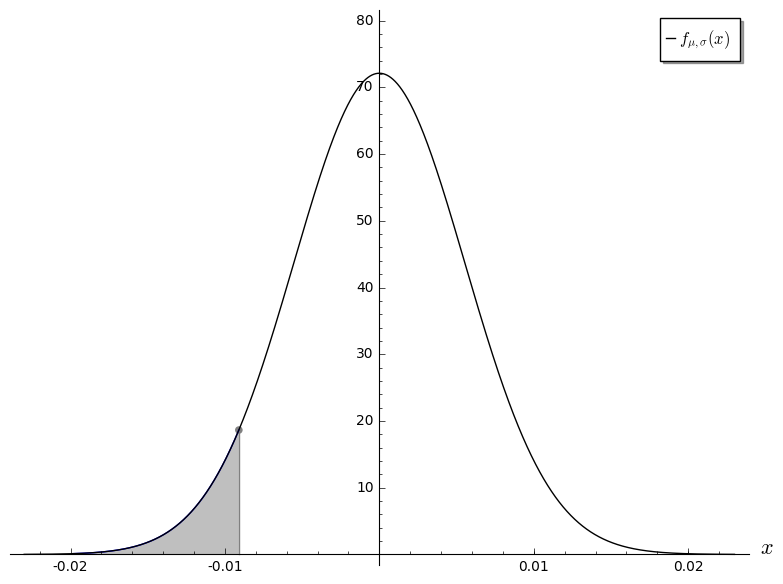
\includegraphics[scale=0.5]{chart1.png}
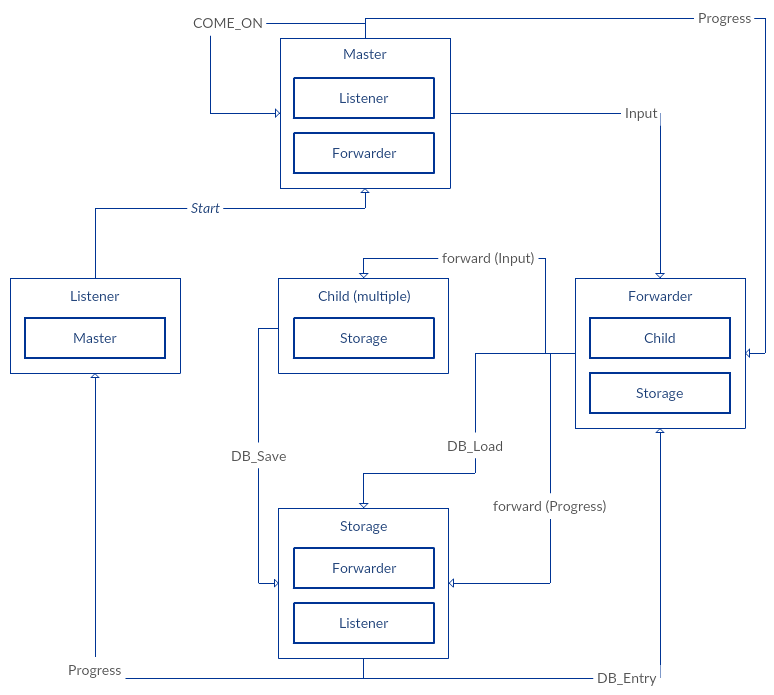
\includegraphics[scale=0.5]{akka.png}
\end{center}
\caption{Diagram przepływu wiadomości między aktorami} %\label{czynnosci_GD}
\end{figure} 

\subsubsection{Aktor \textit{Listener}}
Tworzony jest jako pierwszy aktor w całym systemie. Jego głównym zadaniem jest nasłuchiwanie postępu prac pozostałych aktorów oraz komunikatów o ich ewentualnych awarii.

\subsubsection{Aktor \textit{Master}}
Tuż po \textit{Listenerze} powoływany do życia jest aktor typu \textit{Master}. Możliwe jest zadanie \textit{Masterowi} zapytania przez użytkownika systemu, jak na przykład wyliczanie $VaR$ ze zwiększoną precyzją (standardowa precyzja to 10000 symulacji dla portfela), ewentualnie zmniejszenie precyzji w celu szybkiego uzyskania
wyniku.

\textit{Master} wysyła wiadomość z parametrami do pośrednika (klasa \textit{Forwarder}). Warto nadmienić, że wysyłając tę wiadomość Master korzysta z konstrukcji \textit{ask()}. Wysyłana jest wiadomość, ponadto tworzony jest obiekt typu \textit{Future}, który jest reprezentacją odpowiedzi adresata. \textit{Future} pozwala nam operować na potencjalnych odpowiedziach które jeszcze nie nadeszły. Dzięki temu można zaimplementować przetwarzanie potokowe (ang. pipeline processing), ponieważ na obiekcie \textit{Future} można przeprowadzać obliczenia,
zarówno funkcjami nazwanymi jak i anonimowymi. W tym konkretnym przypadku mapujemy (używając klasy \textit{Mapper}) obiekt reprezentujący portfel z parametrami na obiekt będący wynikiem dotychczasowych prac aktorów – który następnie trafia do \textit{Listenera}.


\subsubsection{Aktor \textit{Forwarder}}
Pośrednik po otrzymaniu portfela, w zależności od tego czy aktorzy klasy \textit{Worker} są już dostępni, decyduje o rozdzielaniu porcji, czyli dobieraniu liczby symulacji przypadającej na jednego aktora klasy \textit{Worker}.

Gdy aktorzy klasy \textit{Worker} nie są jeszcze dostępni, lub z innego powodu są niezdolni do pracy, \textit{Forwarder} podejmuje starania by stworzyć nowych aktorów, ale zanim to uczyni, wywołuje  procedurę zapisującą tymczasowo portfel we własnej pamięci (\textit{backlog}).


\subsubsection{Aktor \textit{Worker}}

Każdy \textit{Worker} jest aktorem potomnym \textit{Forwardera}. Po uszkodzeniu aktora potomnego to właśnie aktor nadrzędny, zwany również obserwatorem (ang. \textit{Supervisor}), podejmuje decyzję co należy uczynić. W tym konkretnym przypadku \textit{Forwarder} używa standardowej strategii systemu \textit{Akka}, tj. \textit{OneForOneStrategy}.
Strategia ta zakłada, że awaria jednego z aktorów potomnych nie powinna mieć
wpływu na pracę pozostałych. Uszkodzony aktor zostaje zatrzymany przez
obserwatora, a następnie obserwator tworzy nowego aktora, który otrzymuje to
samo zadanie któremu poprzedni aktor potomny nie podołał.

Worker ma za zadanie na podstawie portfela i jego parametrów wyliczyć odpowiednią ilość wektorów skorelowanych względnych zmian cen $Y(k)$ - wg. równania \eqref{eq:ynk}.












\newpage
\bibliographystyle{plain}

\bibliography{P2P}
Philip Best, Wartość narażona na ryzyko, tłum. Andrzej Komański,
\\
Kraków 2000 ISBN: 82-88597-01-9.

\end{document}
